\documentclass[a4paper]{article}
\usepackage[left=3cm, right=3cm]{geometry}
\usepackage{hyperref}
\usepackage{cite}
\usepackage{amssymb}
\usepackage{url}
\usepackage{float}
\usepackage{longtable}
\usepackage{array}
\usepackage{algorithmic}
\usepackage[boxed]{algorithm}
\usepackage{color}
\usepackage{graphicx}
\usepackage{tabularx}
\usepackage{caption,subcaption}
\pagestyle{headings}
\newcommand{\secondo}{\textsc{Secondo}}
\newcommand{\bmodb} {BerlinMOD Benchmark}
\newcommand{\op}[1]{\textbf{#1}}
\newcommand{\dt}[1]{\textsl{\underline{#1}}}
\newcommand{\true}{\textsl{TRUE}}
\newcommand{\false}{\textsl{FALSE}}
\newcommand{\secver}{2.9.StableNewFlob}
%opening
\title{Network Data Model and BerlinMOD Benchmark}
\author{Simone Jandt}
\date{Last Update: \today}
\begin{document}
\maketitle
\begin{abstract}
In the past several data models for the representation of histories of  spatio-temporal data
objects have been developed. Among others we can categorize these data models
into data models for objects moving freely in the two dimensional space and data
models for network constrained moving objects. We selected two representants,
one for each data model category, which are both implemented in the \secondo{} DBMS,
and compared their capabilities with the \bmodb{}. In this paper we present our
translation from the \bmodb{} into the network constrained data model and show
that the network constrained data model outperforms the data model of free movement
in the two dimensional space by orders of magnitudes.

%The very good results of the network data model in this comparsion encourages us
%to propose a extension of the \bmodb{} with a additional query set BerlinMOD/Net.
%This new query set covers the specialised challenges for network constrained
%data models and enables us to use the \bmodb{} to compare the capabilities of
%different network data models with respect to this specialised network challenges.
\end{abstract}
\section{Introduction}
In the past several data models for the representation of spatial and
spatio-temporal data objects have been developed. Among others we can categorize
them into data models for objects moving freely in two dimensional space and
data models for network constrained moving objects. For both categories
several different data models have been presented like
\cite{335426,chenzaniolosqlst} for spatio-temporal data objects moving freely in
two dimensional space and \cite{1146465,956692,VazWolfNetMod} for
spatio-temporal data objects that are constrained by given networks,
to name just a few. Objects which are restricted to use existing networks, like
cars to road networks, can be represented as moving point object in both data
models, while objects, which are not restricted by a given network, like people,
can be represented as moving point object only in the data models of free movement
in space. So, why do we spend time in developing network data models, if the network
constrained moving objects can be represented elsewhere in the data model of free
movement in the space?

We decided to compare the capablities of the both different data models. For our
experiments we choosed one example data model as representative for
each of the both categories. Spatio-temporal objects moving freely in the two
dimensional space are represented by the data model presented in \cite{335426}.
And network constrained data models are represented by the network data model
presented in \cite{1146465}. We choosed this two representatives, because both
data models are available in the \secondo{} DBMS and use the same temporal
representation. So we can exclude that the use of different DBMS or temporal
representations bias the results of our comparision.

As we use \secondo{} it seems to be a logical next step to use the \bmodb{}
\cite{BerlinMODVLDB} to compare the capabilities of the
both data models. The \bmodb{} is best to our knowledge the first benchmark for
complete spatio-temporal database systems and it is also available in the \secondo{}
DBMS. Furthermore the \bmodb{} data model is the data model of freely movement
in two dimensional space that we use for our comparison. So we only have to
transform the \bmodb{} spatial and spatio-temporal data types once into our
network data model representation. This avoids sources of errors in transformation
and makes it more easy to control the query results for correctness. Furthermore
the data generated by the \bmodb{} data generator is restricted to the streets of the
German capital Berlin, such that it can be translated into a network data model
environment.

In this paper we describe the transformation of the \bmodb{} benchmark data and
queries into network data model representation. And show that the network data
model outperforms the data model of free movement in space significantly in our
experiments. The network data model uses less than 60\% of the storage space of
the data model of free movement in space, mostly caused by the fact that the number
of units for the moving point objects in the network data model is less than 50\% of
the number of units in the data model of free movement in space. The total run times
for the \bmodb{} of the network data model is less than 50\% of the total run time
of the data model of free movement in space. We think that this results show that
it is useful to develope specialised data models for network constrained moving objects
to save storage space and reduce query run times.

%The very good results of the network data model encourages us to propose the extension
%of the \bmodb{} by a query set BerlinMOD/Net. The new query set covers the specialised
%challenges of network data models like network distance computing which are not
%covered by the original \bmodb{}. The new query set should enable us to compare
%the capabilities of different network data models with respect to the special
%challenges of network constrained data models.

The rest of the paper is organised as follows: In section \ref{sec:relWork} we give a
short reminder of the underlying \secondo{} DBMS (\ref{sec:secondo}), the \bmodb{}
(\ref{sec:bmodb}) and the two data models (\ref{sec:bmodbdatamod}
and \ref{sec:netdatamod}) we choosed as representatives for our comparision.
The translation of the \bmodb{} data and query set in the network data model
representation is described in section (\ref{sec:Translation}). The resulting
experimental benchmark setup is described in section \ref{sec:scenario} followed
by the results of our experiments in section (\ref{sec:results}).
%At least we present our proposed extension of the \bmodb{} for network data models in
%section \ref{sec:newqueries}.
We conclude our work in section \ref{sec:summary}.
\section{Related Work}
\label{sec:relWork}
In the past other data models for free movement in the space
\cite{335426,chenzaniolosqlst} and for network constrained movement have been
presented \cite{1146465,956692,VazWolfNetMod}. As well there are some more
benchmarks \cite{COSTBenchmark, QueriesTheodoridis} and database systems for
spatial and spatio-temporal datatypes \cite{HERMES,1054151}. But best to our
knowledge they don't actually provide a combination of different implemented
and supported data models together with a existing benchmark feasible for moving
objects in space and network constrained moving objects like the actual
\secondo{} DBMS. So it is self-evident for us to use the \secondo{} DBMS in
combination with the provided data models and the \bmodb{} to compare the
capabilities of the network constrained data model and the data model of free
movement in spache provided with the \secondo{} DBMS.

In the next subsections we give short reminders of the \secondo{} database system
(\ref{sec:secondo}), the \bmodb{} (\ref{sec:bmodb}), and the both data models
(\ref{sec:bmodbdatamod}, \ref{sec:netdatamod}) we used in our experiments.
\subsection{Secondo}
\label{sec:secondo}
The extensible \secondo{} DBMS presented in \cite{686903,1054151} provides a
platform for implementing various kinds of data models. It provides a clean
interface between the data model independent system frame and the content of the
single data models. Hence \secondo{} can be easily extended by the user
implementing algebra modules to introduce  new data types and operations on
this data types. The user may define additional viewers for the graphical user
interface or write additional optimization rules or cost functions to extend the
the optimizer. Since \secondo{} version 2.9 the user may publish his extensions
as \secondo{} plugin such that other users can use this plugin to extend their own
\secondo{} system to use the functionalities or repeat the published experiments.
\secondo{} is free available in the web \cite{secondoweb} and comes with a number
of already implemented spatial and spatio-temporal data types
and operations including the spatio-temporal data model of free movement in the
two dimensional space \ref{sec:bmodbdatamod} and the network data model
\ref{sec:netdatamod} used in our work. Furthermore the \bmodb{} described in
\ref{sec:bmodb} has been developed in the \secondo{} DBMS. For our experiments
we used the \secondo{} version \secver{}.
\subsection{BerlinMOD Benchmark}
\label{sec:bmodb}
The \bmodb{} was presented in \cite{BerlinMODVLDB} \nocite{BerlinMOD} and the
provided scripts for the data generator are implemented as \secondo{} DBMS operations.
The \bmodb{} is available in the web \cite{berlinmodweb} and provides a well defined
data-set and queries for the experimental evaluation of the capabilities of
spatial and spatio-temporal database systems dealing with histories of moving
objects. The \bmodb{} emphasises the development of complete systems
and simplifies experimental repeatability pointing out the weakness and the potencies
of the benchmarked systems.

The data-sets of the \bmodb{} are created using the street map of the German
captial Berlin \cite{bbike} and statistical data about the regions of Berlin
\cite{bevberlin,berlinstadtatlas} as input relations.
The created moving objects represent cars driving in the streets of Berlin,
simulating the behaviour of people living and working in Berlin.
Every moving object has a home node and a work node. Every weekday each car will
do a trip from the home node to work the work node in the morning and vice versa
in the late afternoon. Besides this randomly choosen cars will make additional
trips in the evening and up to six times at the weekend to randomly choosen
targets in Berlin. The \bmodb{} uses the data model of free movement in two
dimensional space described in section \ref{sec:bmodbdatamod}. Because the \bmodb{}
generates all data sets restricted to the street map of Berlin the \bmodb{} can
also be used for network constrained data models, if the spatial and spatio-temporal
data types are translated into a corresponding network data model, like we did
for our experiments.

The number of observed cars and the duration of the observation period can be
influenced by the user setting the $SCALEFACTOR$ to different values in the data
generation script of the \bmodb{}. For example at $SCALEFACTOR$ 1.0 the data generator
creates 2000 moving point objects observed for 28 days. Each of them sending a
GPS-signal every 2 seconds. This simulated signals are simplified such that time
intervals when a car doesn't move or moves in the same direction at the same
speed are merged into one moving unit. This means that, if a car stays in front
of the work node for 8 hours there will be only one entry in the cars
history of movement with a time interval of 8 hours instead of 14.400 entries
one for each GPS interval.

The \bmodb{} provides two different approaches to store the histories of moving
objects. On the one hand the object-based approach (OBA) and on the other hand
the trip based approach (TBA).

In the OBA the complete history for each moving object is kept together into
one single entry. There is only one relation $dataScar$
containing one tuple for each object consisting of the spatio-temporal data of
the object $journey$, the $licence$, the $type$, and the $model$ of the object.

In the TBA we have two relations $dataMcar$ and $dataMtrip$. $dataMcar$ contains
the static data for each object like $licence$, $type$, and $model$ together with
an object identifier $moid$. $dataMtrip$ contains for each $moid$ several tuples
each of them containing all units of a single trip of the moving object or a
single unit for a longer stop. For example each time the car drives from home node
to work node is a single trip and each time the car parks in front of the office
is also a single trip.

Besides the moving objects the \bmodb{} provides several data sets each of them
containing 100 pseudo randomly generated data objects which are used in the
benchmark queries. Table \ref{tab:queryobjects} gives an overview of this query
objects.

\begin{table}[H]
  \begin{tabularx}{|l|X|}
    \hline
    \textbf{Name of Data Set}&\textbf{Tuple Content}\\
    \hline
    $QueryPoints$&Object identifier and \dt{point} values.\\
    \hline
    $QueryRegions$&Object identifier and \dt{region} value.\\
    \hline
    $QueryInstants$&Object identifier and time stamps.\\
    \hline
    $QueryPeriods$&Object identifier and space of time.\\
    \hline
    $QueryLicences$& Object identifier and a \dt{string} representing a licence value.\\
    \hline
  \end{tabularx}
  \caption{Query Object Relations of \bmodb{}}
  \label{tab:queryobjects}
\end{table}

The \bmodb{} provides two sets of queries BerlinMOD/R and BerlinMOD/NN.
BerlinMOD/R addresses range queries and BerlinMOD/NN nearest neighbour queries.
In this paper we will focus on the range queries, which are the main aspect of the
\bmodb{} up to now.

The query set BerlinMOD/R includes 17 queries selected of the set of possible
combinations of the 5 aspects:
\begin{itemize}
  \item object identity (known / unknown),
  \item dimension (standard / spatial / temporal / spatio-temporal),
  \item query interval (point / range / unbounded),
  \item condition type (single object / object relations),
  \item aggregation (with or without aggregation).
\end{itemize}
We will present the 17 queries in more detail in section \ref{sec:queries}
together with our network data model translation of this queries.
\subsection{Data Model of Free Movement in 2D space}
\label{sec:bmodbdatamod}
The data model used by the \bmodb{} is the same data model of freely moving in
two dimensional space presented in \cite{594784,335426,352963}. Spatial
positions are assumed to be located into a two dimensional space. A single spatial
position is represented by the data type \dt{point}. A \dt{point} consists of a pair of
\dt{real} values interpreted as x,y-coordinates in the assumed two dimensional plane.

Streets are represented by \dt{line} values. A \dt{line} value consists of a set
of $half segments$ representing the geometry of the line in the two dimensional space.
Each $half segment$ consists of two \dt{point} values and a boolean value telling
if the left or the right point is the dominating point of the $half segment$.

Regions are represented by the data type \dt{region}. A \dt{region} consists of
a set of $half segments$ defining the outer border of the region in
the two dimensional space. If a region contains wholes the inner border is also
formed by the $half segments$.

In \secondo{} all this spatial data types and many standard data types can be
lifted to become time dependent \dt{moving} values. For all data types \dt{$\alpha$}
the constructor \dt{moving} creates a new data type \dt{moving}(\dt{$\alpha$})
(short form \dt{m$\alpha$}).

A car may be represented by a \dt{mpoint}. A \dt{mpoint} is a \dt{point} object changing
its value within time. Therefore a \dt{mpoint} consist of a set of units called
\dt{unit}(\dt{point}) (short form \dt{upoint}). Each \dt{upoint} consists of a time
interval and two \dt{point} values. The first \dt{point} value represents the
position of the \dt{mpoint} at the start of the time interval and the second
\dt{point} value represents the position of the \dt{mpoint} at the end of the
time interval. It is assumed that the point moves on the straight line between
this two points with constant speed, which is defined by the ratio from the
distance of the two points and the length of the time interval of the unit.
All units of a \dt{mpoint} must have disjoint time intervals, because a car
cannot be at two different positions at the same time.
The units are sorted by ascending time intervals.

This spatio-temporal data model of \dt{moving} allows us to compute the position
of a \dt{mpoint} at every time instant within its definition time.
We can also compute the time instant the point passed a
given position assumed the \dt{mpoint} ever passes this position. The position of a
\dt{point} at a given time instant is represented by a \dt{intime}(\dt{point})
(short form \dt{ipoint}). A \dt{ipoint} consists of a time instant and a \dt{point} value.

Some other data types of \secondo{} which are used in the \bmodb{} are shown in
table \ref{tab:bmodbdatatypes}.
\begin{table}[H]
\begin{center}
\begin{scriptsize}
\begin{tabularx}{\textwidth}{|l|X|}
\hline
\textbf{Data Type} & \textbf{Description} \\
\hline
\dt{bool} & Usual boolean data type.\\
\hline
\dt{int} & Usual integer number.\\
\hline
\dt{real} & Usual real number.\\
\hline
\dt{instant} & A point in time.\\
\hline
\dt{periods} & A set of disjoint and not connected spaces of time.\\
\hline
\dt{mbool} & A time dependent boolean value, which will be constant \true{} or \false{}
within each \dt{ubool} \\
\hline
\dt{mreal} & Time dependent real number. Each unit will be defined by a function
of time representing the \dt{real} value at each time instant.\\
\hline
\end{tabularx}
\end{scriptsize}
\caption{Other Data Types of \bmodb{}}
\label{tab:bmodbdatatypes}
\end{center}
\end{table}
\subsection{Network Data Model}
\label{sec:netdatamod}
The central idea of the network data model presented in \cite{1146465} is that
every movement is constrained by a given network and every position can be described
relative to this network. This make the data type \dt{network} to the central
data type in the network data model. All other data types of the network data model
are related to a given \dt{network} object by the unique network identifier that
is part of each \dt{network} object.

The \dt{network} object contains all spatial informations of the represented network
in three main relations, two sub relations and some indexes to support faster
access to the relations.

The relation $routes$ contains the attributes of the
streets like $id$, $route curve$, $route length$, and two boolean flags. The first
flag indicates if the route starts at the lexicographically smaller end point or not.
The second flag indicates if the lanes of the street are separated like on German
Highways or not.

The $junctions$ relation contains all attributes of the street
crossings like the two route identifiers of the first and second street meeting at the
crossing, the distance of the crossing from the start of the first respectively
second street, tuple identifiers of the both streets in the routes relation,
tuple identifiers of the sections connected by this junction in the sections relation,
and a connectivity code telling us which lanes of the two streets are connected
by the crossing.

The $sections$ relation of the \dt{network} object contains the
attributes of the street parts between two crossings or a crossing and
the end of the street. This are the route identifier of the street the section
belongs to, the tuple identifier of this street in the routes relation, the start
position and end position of the section on the street, the section curve, and
again two boolean flags with the same meaning as in the routes relation.

Furthermore there are two arrays in the \dt{network} object providing a fast
access from each section to their adjacent sections with respect to the driving
direction. Two sections are adjacent if their lanes are connected by a junction.

We created four B-Tree indexes for the route identifier attributes in the $routes$,
$junctions$ and $sections$ relation, and a R-Tree index over the curve attribute
of the $routes$ relation to support faster execution of operations dealing with
the relations of the \dt{network} object.

The data type \dt{gpoint} represents single positions in a given network. Besides the
network identifier a \dt{gpoint} consists of a route identifier, a distance from
the start of the route to the position of the \dt{gpoint} and a $side$ value
({$up$, $down$, $none$) telling us if the position is reachable from the $up$
or the $down$ side of the route in case of seperated lanes. For simple
streets or positions which are reachable from both sides of the route the side
value is always $none$.

Parts of the network, regardless if they represent paths or regions, are given as
\dt{gline} values. Besides the network identifier a \dt{gline} consists of a set
of $route interval$s, and two boolean flags. The boolean flags tell us if the
\dt{gline} is defined and if the set of $route interval$s is sorted.

Each $route interval$ consists of a route identifier identifying the route
the route interval belongs to, and the start and the end position from the
route interval on this route
\footnote{In the original paper the $route interval$ includes a $side$ value
analogous to the \dt{gpoint}. But this parameter is not part of the implementation yet.}.
We call a \label{sec:sortedgline} set of $route interval$s sorted if the following
conditions are fullfilled:
\begin{itemize}
	\item all $route interval$s are disjoint
	\item the $route interval$s are stored in ascending order of their route identifiers
	\item if two disjoint $route interval$s have the same route identifier the
$route interval$ with the smaller start position is stored first
	\item for all $route interval$s the $startPosition \le endPosition$
\end{itemize}
Many algorithms take profit from sorted \dt{gline} values. For example: If $n$
is the number of the route intervals in the \dt{gline} the
decision, if a \dt{gpoint} is inside a \dt{gline} needs O($n$) time for unsorted
and O($\log n$) time for sorted \dt{gline} values,

Unfortunately not all \dt{gline} values can be stored sorted. If a \dt{gline}
value represents a path between two \dt{gpoint} in the network, we need the
route intervals exactly in the sequence they are used in the path. This will
nearly never be a sorted set like defined before. We solved this dilemma by
introducing the boolean sorted flag. Every algorithm which can take profit from
a sorted \dt{gline} checks this flag and uses the corresponding code. We store \dt{gline}
values sorted whenever this is possible to support faster query execution.

Mostly similar to the \dt{mpoint} of the other data model there is a
\dt{mgpoint} in the network data model. A \dt{mgpoint} consists of a set of
\dt{ugpoint} with disjoint time intervals. Each \dt{ugpoint} consists of a time
interval and two \dt{gpoint} values. Every time the \dt{mgpoint} changes the route
or the speed a new \dt{ugpoint} is written. Each \dt{ugpoint} is assumed to follow
the same route from the start to the end position at the same speed. So accordingly
to the \dt{mpoint} we can compute the network position of the \dt{mgpoint} at every
time instant within the definition time of the \dt{mgpoint} as \dt{intime}(\dt{gpoint}).

In deviation from the original network data model we extended the implementation
of the \dt{mgpoint} with four additional attributes to support faster query execution:
\begin{enumerate}
	\item The total driven distance
	\item A sorted set of $route interval$s representing the positions ever
traversed by the \dt{mgpoint}
	\item A boolean defined flag for the set of route intervals
	\item A spatio-temporal minimum bounding box
\end{enumerate}
The sorted set of $route interval$s was introduced, because it makes it much
faster to decide if a \dt{mgpoint} ever passed a given network position or not.
Instead of a linear check of all $m$ \dt{ugpoint}s of a \dt{mgpoint} we can
perform a binary scan on the much lower number $r$ of the passed $route interval$s.
This reduces the time complexity from O($m$) to O($\log r$) for all \op{passes}
operations. Logically the set of $route interval$s should be a sorted \dt{gline}
value but the \secondo{} DBMS restricts us to use a sorted set of $route interval$s
instead.

The spatio-temporal minimum bounding box was introduced as parameter to the
\dt{mgpoint} because the computation of this value is very expensive in the
network data model. Although each unit of a \dt{mgpoint} stays on the same route
at same speed it may follow different spatial directions. For example a route may
lead uphill in serpentine. A spatial bounding box only computed from the spatial
start and end position may not enclose all spatial positions of the car within
the unit. Therefore we have always to examine the spatial dimensions of the
$route interval$ passed within a unit to compute the units bounding box. This
needs a access to the route courve in the $routes$ relation of the corresponding
\dt{network} object. If $r$ is the number of routes
of the network and $h$ the number of $half segments$ belonging to the $route interval$
passed in a unit we need O($h + \log r$) time to
compute the bounding box for a single unit. The bounding box of the \dt{mgpoint}
is the union of the bounding boxes of its $m$ units. So the computation of the
spatio-temporal respectively spatial bounding box of a \dt{mgpoint} needs
O($m(h + \log r)$) time. This very expensive bounding box computation is only done
on demand or if we can get the bounding box for free. For example we can copy
the bounding box of a \dt{mpoint} at the translation time into a \dt{mgpoint}
without big computational costs. The bounding box attribute is not maintained. If
the \dt{mgpoint} value changes the bounding box attribute is set to be undefined
until its recomputation is necessary.
\section{Translation of BerlinMOD into Network Data Model}
\label{sec:Translation}
First of all we describe the creation of the \dt{network} object from the $streets$
value of the \bmodb{} in section \ref{sec:createNetwork}. Then we describe how
to use this new created \dt{network} value as reference for the translation of
all spatial and spatio-temporal data objects of the \bmodb{} into the network data
model representation in section \ref{sec:translateSTdata}.
In section \ref{sec:createIndex} we describe the indexes we build on the network
data model representation to support faster query execution.
In section \ref{sec:queries} we describe the executable \secondo{} queries for the
network data model representation of the \bmodb{}.

Executable \secondo{} scripts for the network and index creation, object translation,
and the executable benchmark queries can be downloaded from our website
\cite{berlinmodweb}.
\subsection{Create Network Object}
\label{sec:createNetwork}
The \dt{network} object $net$ is created by extracting the $routes$ data from
the $streets$ object that is created by the BerlinMOD Data Generator.
The extracted data $r$ is used to compute the crossings of the
routes of Berlin $j$. The data source lacks on information about the connectivity
of the street crossings, such that we use the maximum value for the connectivity
code of each crossing as default value in this step.
Now we can use $r$ and $j$ as input relations for the operator \op{thenetwork}
to create our \dt{network} object $net$ representing the streets of Berlin in
the network data model representation of the \bmodb{}.

The network creation algorithm first copies all tuples of $r$ to the
$routes$ relation of $net$ and creates the B-Tree index of the route
identifiers and the R-Tree index of the route curves of the $routes$ relation of
$net$. Then all tuples of $j$ are copied to the $junctions$ relation
of $net$ and the tuple identifiers for the both routes connected
by this junction are added to the junctions entry. After that we build two B-Trees
indexing the route identifiers of the first respectively second route in the
$junctions$ relation. Next for every route of the $routes$ relation all junctions
on this route are taken from the $junctions$ relation to compute the up and
down sections for each of this junctions on the route. The up and down
sections are inserted into the $sections$ relation of $net$ and the
tuple identifiers of the sections are added to the entry of the corresponding
junction in the $junctions$ relation. After that the B-Tree index for the
route identifiers in the $sections$ relation is created and the adjacency
lists of $net$ are filled with the adjacent section pairs defined by the
$junctions$ relation.

If $|r|$ is the number of routes and $|j|$ is the number of junctions.
The algorithm needs O($|r| \log |r|$) time to copy $r$ to the
$routes$ relation of $net$ and create the indexes of the
$routes$ relation. The creation of the $junctions$ relation and the build
of the B-Trees indexes takes O($|j| \log |j|$) time.
O($|r||j|$) time is needed to fill the $sections$ relation and
O($|j|$) time to fill the $adjacency lists$ of $net$. Alltogether
the complete algorithm needs:
O($|r| \log |r|+|j| \log |j| + |r||j|$)
 time to create the $net$ from the two input relations $r$ and $j$.
\subsection{Translate Spatial and Spatio-Temporal Data Types}
\label{sec:translateSTdata}
In this section we describe the translation of the spatial and spatio-temporal
data types of the \bmodb{} data set into network respectivels network-temporal
objects. All translations are done relative to the \dt{network} object $net$ created
before (see  \ref{sec:createNetwork}).
The input for all algorithms is a spatial respectively
spatio-temporal \bmodb{} data object and the \dt{network} object $net$.
All Network translation algorithms return a undefined object if the input data
object is not constrained by $net$.

\subsubsection{Translate \dt{point} into \dt{gpoint}}
We start the explanation of our translation algorithms with the \op{point2gpoint}
operation, because \op{point2gpoint} is used by the other translation algorithms.
The algorithm translates a \dt{point} value $p$ into a corresponding
\dt{gpoint} value $gp$. It uses the R-Tree index of the
$routes$ relation of $net$ to select the route closest to $p$ and computes the
position of $p$ on this route curve. The $side$ value of $gp$ is always set
to $none$. Because the \bmodb{} does not differntiate between the sides of a
road. If $r$ is the number of routes in the $routes$ relation
and $k$ is the number of possible candidate routes the worst case complexity
of the algorithm is O($\log{r} + k$).

This should be all to translate the \dt{point} values of the $QueryPoints$
relation of the \bmodb{} into network query positions. But there is a problem with
the network data model representation of junctions. In the network data model
contrary to the data model of freely moving in space junctions have more than one
\dt{gpoint} representation, because they are related to two or more routes. Hence
if a junction position is given related to route $a$ we won't detect the
junction as passed if a \dt{mgpoint} object passes the junction on route $b$
in all cases, because the definition of \op{passes} in the network data model is
slightly different from the \op{passes} operation in the \bmodb{} data model.
Unfortunately all query points of the \bmodb{} are junctions. As work around we
added a operator \op{polygpoints}, which returns for every input \dt{gpoint}
value $gp$ a stream of \dt{gpoint} values. If $gp$ represents a junction
we return all \dt{gpoint} values representing the same junction in $net$,
otherwise we return only $gp$ in the stream. So we got 221 query \dt{gpoint}
values in $QueryPointsNet$ for the 100 query \dt{point} values in
$QueryPoints$ and 22 \dt{gpoint} values in $QueryPoints1Net$ for the
10 \dt{point} values of $QueryPoints1$ of the \bmodb{}. This means we have
always to compute the results for the doubled number of query points in our network
data model than in the data model of free movement in space.

\subsubsection{Translate \dt{mpoint} into \dt{mgpoint}}
The second operation \op{mpoint2mgpoint} translates a \dt{mpoint} value $s$
into a \dt{mgpoint} value $t$. The main idea of the algorithm is to use the
continuous movement of $s$ to reduce computation time. We initialize the
algorithm by reading the first unit of $s$ and use the \op{point2gpoint}
algorithm to find a route in the network containing the $start$ and
the $end point$ of this unit. We initialize the first unit of $t$ with
the computed network values. Then we read the next unit of $s$ and try to find
the $end point$ of the new unit on the same route the last unit of $s$ was
found. If the $end point$ is found on the same route we check the direction and
speed of the point in the unit. If they are equal to the actual unit we extend
the actual unit of $t$ to enclose the value of the actual unit of $s$. If the
speed or the moving direction changes we write the actual unit to $t$ and initialize
a new unit for $t$ with the network values of the actual unit from $s$.
If the $end point$ can't be found on the same route than the last unit from
$s$ we write the actual unit of $t$ and start a search on the route curves
of the adjacent sections to find the route curve that contains the $start$
and the $end point$ of the actual unit of $s$. We initialize a new unit
for $t$ with the estimated network values for the actual unit of $s$ and
continue with the next unit of $s$. At last we add the actual network unit
to $t$.

The time complexity to find the start values for the first unit is O(\op{point2gpoint}).
For the next $m$ units of $s$ the time complexity is O(1) if $s$ don't change the
route. And O($a$) if the end point is on another route and $a$ is the maximum
number of adjacent sections. So we get a worst case time complexity of
O(O(\op{point2gpoint}) + $ma$) for the translation of a \dt{mpoint} $s$ into a
\dt{mgpoint} $t$.

\subsubsection{Translate \dt{region} into \dt{gline}}
The translation of the \dt{region} values in the $QueryRegions$ relation of the
\bmodb{} into \dt{gline} values of our network data model is done in several steps.
First of all we build a single big \dt{line} object containing all network streets.
Then we compute for each \dt{region} of the $QueryRegions$ the intersection with
this big \dt{line} object. At last we translate the resulting \dt{line} objects
of the intersection, each representing one \dt{region} of the $QueryRegions$
relation, into sorted \dt{gline} values using the \op{line2gline} operation.

The algorithm of the \op{line2gline} operation takes each $half segment$ of a
\dt{line} value and computes a corresponding network $route interval$ by
searching a common $route curve$ for the $start$ and the $end point$ of the
$half segment$ using the \op{point2gpoint} operation. The computed
$route interval$s are sorted, merged and compressed before the resulting
\dt{gline} value is returned. If the number of $half segment$s of a \dt{line}
value is $h$ and the number of resulting compressed $route interval$s is $r$
we get a time complexity of O($h$O(\op{point2gpoint})$+ h \log r + r$) for the
whole algorithm. Whereby the summand $h \log r + r$ is caused by the compressing
and sorting of the resulting \dt{gline} but as mentioned before
in \ref{sec:sortedgline} we think this time is well invested, because it is needed
once and the sorted \dt{gline} value is used many times.
\subsection{Create Indexes on Network Data Model}
\label{sec:createIndex}
For the use with the \bmodb{} we created the following indexes on the network
data model representation of the \bmodb{} data sets:
\begin{itemize}
  \item B-Tree indexes for the $licences$ and $moid$ attributes of the relations
$dataSNcar$, $dataMcar$, and $dataMNtrip$. This indexes are similar to the indexes
created in the \bmodb{} for $dataSCcar$, $dataMCcar$, and $dataMCtrip$, because
the relations $dataSNcar$, $dataMcar$ and $dataMNtrip$ contain the network
data model representation of the $dataScar$, $dataMcar$ and $dataMtrip$ relation
of the \bmodb{}, such that we don't explain them in more detail.
  \item An R-Tree index of the spatio-temporal bounding boxes of the \dt{mgpoint}
attributes in the $dataMNtrip$ and the $dataSNcar$ relation. Different from the
data model that uses the spatio-temporal units for the spatio-temporal indexes we
used only the big bounding boxes of the whole trips.
 \item For every unit of each \dt{mgpoint} we build a three dimensional $netbox$
and for every $route interval$ of every \dt{mgpoint}s trajectory a two dimensional
$netbox$. This $netboxes$ are used to create R-Trees indexing the network and
network-temporal positions of the \dt{mgpoint}s. A temporal-network bounding box
is a degenerated three dimensional rectangle. The coordinates are defined to be
$x_1 = x_2 = route identifier$ as \dt{real} value (The equality of $x_1$ and
$x_2$ makes the degeneration.), $y_1 = \min (star position, end position)$,
$y_2 = \max (start position, end position)$,
and, $z_1 = starttime$ as \dt{real} value and $z_2 = endtime$} as \dt{real} value.
The network bounding boxes are defined to be degenerated two dimensional rectangles
with x,y-coordinates analogous to the temporal-network boxes.
\end{itemize}
\subsection{Translate Benchmark Queries}
\label{sec:queries}
We developed executable \secondo{} queries for each of the 17 BerlinMOD/R queries
for the object based approach (OBA) and the trip based approach (TBA) using our
network indexes to support faster query execution. The optimization has to be
done manually because the \secondo{} optimizer is not able to optimize SQL-queries
on network data model objects yet. In our experiments we tried many different query
formulations for each query to get optimal queries delivering the correct result
in a minimum of time. The limited space does not allow us to show all our
executable \secondo{} network queries in detail but the \secondo{} scripts with
the complete network data model query sets can be downloaded from our webpage.
In the following we describe only the algorithms of a few queries in detail.

Every time we need a licence in the result or have a query licence number we need
a additional step in the TBA. Because we have to join the $dataMNtrip$ and $dataMNcar$
relation using the $moid$ attribute and the corresponding B-Tree indexes.
We will not repeat this step at every single query description.

Query 1 and 2 work only on standard attributes. They are formulated analogous to
the original queries of the \bmodb{} only the relation names and the used B-Trees
are changed to match the network data model.

Query 3 uses the licence B-Tree to select the ten cars with licences from
$QueryLicences1$ from $dataSNcar$ then the positions of this cars are computed
for each of the ten time instants from $QueryInstants1$.

In Query 4 we produce a two dimensional $netbox$ for each \dt{gpoint} value in
$QueryPointsNet$ and use our specialized netbox R-Tree of the \dt{mgpoint}
$route interval$s to select the passing vehicles.

The queries 5, 6, and 10 retranslate intermediate results into spatial
respectively spatio-temporal objects of the \bmodb{} data model to compute the
Euclidean Distance between this objects. This is done because Euclidean Distances
are not very useful in network environments. In Networks all objects are restricted
to use network paths. Therefore in networks regulary the Network Distance between
objects is computed. To make the results comparable we retranslate the intermediate
results of our network data model into spatial and spatio-temporal data types
and use the existing spatial and spatio-temporal Euclidean Distance Functions of
the \bmodb{} data model for the distance computation in the queries 5, 6, and 10.

Query 5 selects the cars with $licences$ from $QueryLicence1$ respectively
$QueryLicences2$  using the B-Tree over the $Licence$ attribute of $dataSNcar$
and creates a \dt{line} value from the list of $route interval$s passed by
every car. Then the Euclidean Distance between this \dt{line} values is computed
for each pair of licences one from $QueryLicences1$ and one  from $QueryLicences2$.
In the TBA we need a aggregation step building the union of the several
\dt{mgpoint} belonging to each candidate car. This is done with the $route intervals$
returned as trajectory of the \dt{mgpoint} values because it takes much less
time to build the union of the $route intervals$ than of the units of the
\dt{mgpoint} values or the $half segment$s in the \dt{line} values covering the
same network part.

Query 6 uses the \op{filter} operation to select the ''trucks`` from $dataSNcar$
relation, respectively $dataMcar$ relation in the TBA. Then the spatio-temporal
bounding box of each trip is computed and the spatial dimensions of this box are
extended by 5m in every spatial direction. After that the \dt{mgpoint} values are
retranslated into \dt{mpoint} values. In a second step each result of the first
step is joined with all other results of the first step where the extended bounding
boxes intersect, the licences are different and the \dt{mpoint} values have sometimes
a distance lower than 10m. The licence pairs of trucks fullfilling this predicate
are returned. In the TBA there might be duplicate licence pairs which we have to
be removed before we return the result.

The first part of the first step of query 7 is almost equal to the selection of cars
passing a query point in query 4. The intermediate result is filtered to remove all
``not passenger'' cars and for every remaining trip the time the trip reaches first
the query position is computed for every query position and every candidate trip. In
a second step the resulting time instants are grouped by the $id$ of the query
positions and the minimum time stamp of each group is computed. This minimum time
stamp is for every query position the first time it was reached by a car. In the
last step the licences of the cars reaching the query positions at this
first time instant are computed by a join of the results of the first two steps by
query position id and the equality of the time stamps.

In query 8 we just select the candidate cars with the licence B-Tree and compute for
every car the length of the trip at the query periods in the OBA. In the TBA we have
to aggregate over all the distances driven in the single trips by a car within a
query period.

For query 9 we compute the length of every trip in every query period, and select the
maximum driven distance for every period. In the TBA again we have to do a
aggregation of the distances driven from the same car in the same period.

For query 10 in OBA we first retranslate every \dt{mgpoint} value of $dataSNCar$ into
a \dt{mpoint} value and extend the spatial bounding box of each of this
trips by 1.5 m in every direction. Second we select the ten candidate trips given by
$QueryLicences1$, retranslate them and extend their spatial bounding boxes. Than we
join all trips from the first and the second step where the
extended bounding boxes intersect. We filter the pairs that have different licences
and are sometimes nearer than 3m. For this pairs we compute the position of the
\dt{mgpoint} at the times the distance between the both \dt{mpoint} has been smaller
than 3 m. We return the licence pairs and the positions when they have been closer
than 3 m to each other. In TBA we select the trips given by $QueryLicences1$ from
$dataMNtrip$ retranslate them into \dt{mpoint} values. Then we use the
spatio-temporal index of $dataMNtrip$ to select for each of the ten cars the cars
of $dataMNtrip$ which bounding boxes intersect the extended spatio-temporal bounding
boxes of the first selected candidate trips. For every pair of candidate trips we
retranslate the second trip into free movement and use the Euclidean Distance
function for \dt{mpoint} values to determine the deftimes when the both \dt{mgpoint}
had a distance lower than 3m. At least we restrict the trips on this times and
aggregate the resulting trips into one single trip for each licence pair.

In our experiments we tried out several indexes to support faster query execution of
especially of query 10 including the MON-Tree \cite{MONTree}. But at the end this
simple form shows the best complete run time performance of all indexes.

In query 11 we build a network-temporal query box from the product of $QueryInstant$
and $QueryPoints1Net$ relation. And use the network-temporal index on $dataSNcar$
(respectively $dataMNtrip$) to select the resulting trips.

The first step of query 12 is identical with query 11. In a second step a product of
the result of the first step with itself is computed and checked for vehicles which
have been at the same query point at the same query time instant.

Query 13 first computes uses the trajectory value of the \dt{mgpoint} to select the
trips passing a given region. Restricts the trips to the times they pass the region
and tests the resulting trips for their existenz in a given time interval. In TBA
possible duplicate licence pairs have to be removed and the resulting $moids$ must
be mapped to the licences of the cars to generate the result.

Query 14 and 15 build sets of three dimensional network boxes of the query parameters
and use the three dimensional network box tree to select the candidate trips. The
resulting candidate trips are filtered to be sure they realy fullfill the query
constraints.

Query 16 selects the candidate trips using the licence B-Tree, filters them to be
\op{present} within the query periods and restricts them to the times of the
query periods. The restricted trips are filtered with the \op{passes} operation
and restricted to the times they were inside the query region. This is done one time
for $QueryLicences1$ and one time for $QueryLicences2$. The both results are joined
to get the trips of different cars which where at the same period in the same region
without meeting each other there and then in a third step. Again in the TBA we have
to do a additional selection from trips with the $moids$ belonging to the cars
selected before by the licences and to remove duplicates of licence pairs in the
same period.

Query 17 again uses the methods from query 4 to find the trips passing a given query
point. The passing cars are grouped by the passed query points and the number of
cars per query point is computed. In a second step the point with the maximum number
of hits is selected and his id and the number of passing cars is returned. In the
TBA we have to remove the duplicate cars from the result before computing the hits.
\section{Experiments}
\subsection{Setup}
\label{sec:scenario}
For our experiments we used a Standard PC with a AMD Phenom II X4 Quad Core 2.95 GHz CPU,
8 GB main memory, and 2 TB HDD. We used the Linux openSUSE 11.2 operating system and
installed \secondo{} DBMS version \secver{} and the \bmodb{} version provided in the web.

We used the data generating script of the \bmodb{} with $SCALEFACTOR$ values
0.05, 0.2, and 1.0 to generate three data sets in three different database directories.
We used the script ``BerlinMOD\_CreateObjects.SEC'' to create the indexes used by
the data model of free movement in the space. And used our new script
``Network_CreateObjects.SEC'' to create the network data model representation of
the three databases. The script uses the operations and indexes we desribed in
section \ref{sec:Translation} of this paper.

Table \ref{tab:dbstat} shows the created data amounts for the different $SCALEFACTOR$
values. As you can see the network data model needs less than 40\% of the storage
space from the \bmodb{} data model. The main cause is that the same trip is represented
by less than 50\% of the units in the network data model compared to the data
model of free movement in the two dimensional space. We expect this effect to be much
higher if the cars make long distance trips between different towns than in this
experiments, because cars in towns change more often the street and velocity than
cars on long distance trips.
\begin{table}[H]
\begin{center}
\begin{scriptsize}
\begin{tabularx}{1.0\textwidth}{|X|c|c|c|c|c|c|}
\hline
&\multicolumn{2}{c|}{\textbf{Scalefactor 0.05}}&\multicolumn{2}{c|}{\textbf{Scalefactor 0.2}}&\multicolumn{2}{c|}{\textbf{Scalefactor 1.0}}\\
\hline
Number of Cars&\multicolumn{2}{c|}{447}&\multicolumn{2}{c|}{894}&\multicolumn{2}{c|}{2000}\\
\hline
Number of Days&\multicolumn{2}{c|}{6}&\multicolumn{2}{c|}{13}&\multicolumn{2}{c|}{28}\\
\hline
Data Generation&\multicolumn{2}{c|}{164.761s}&\multicolumn{2}{c|}{587.299s}&\multicolumn{2}{c|}{3177.46s}\\
\hline
&BMODB&Network&BMODB&Network&BMODB&Network\\
\hline
Data Translation
and Index Build&301.72s&535.65s&1,362.72s&2,190.45s&7419.130&11,144.13s\\
\hline
Number of Units&2,646,026&1,260,888&11,296,682&5,346,971&52,140,685&24,697,709\\
\hline
Total Storage Space&2.26 GB&0.86 GB&9.51 GB&3.69 GB&45,76 GB&17.28 GB\\
Data&0.79 GB&0.44 GB&3.35 GB&1.83 GB&15.47 GB& 8.40 GB\\
Indexes&1.48 GB&0.42 GB&6.16 GB&1.86 GB&30.30 GB&8.89 GB\\
\hline
\end{tabularx}
\end{scriptsize}
\caption{Database Statistics}
\label{tab:dbstat}
\end{center}
\end{table}
The long creation time for the network data model representation is
caused by the expensive mapping of spatial and spatio-temporal positions into
network positions. The Indexes are build faster in the network representation
because they are much smaller than in the \bmodb{} data representation.

After the data creation we started the benchmark queries for
the object based (OBA) and the trip based approach (TBA) of the \bmodb{} on this
databases and saved the results for each database. Than we formulated executable
\secondo{} queries for each BerlinMOD/R query using the network data model
representation, like described in section \ref{sec:queries} of this paper, and
executed them on the network version of the \bmodb{} database.

We found some isolated missmatches in some query results, when we compared the
results of our network queries with the results of the \bmodb{}
queries to ensure that all results are correct. We detected that the source
data of the street map is not well defined in all places. See figure
\ref{fig:routefailure}) for two examples. We corrected the source file
``streets.data`` delivered by \bmodb{} at the detected places and restarted the
building of the databases and our experiments from the scratch.
\begin{figure}
\begin{center}
   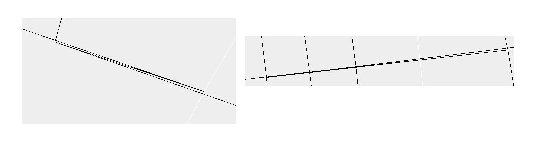
\includegraphics[scale=1.0]{routefailure.eps}
   \caption{Example Failures in Street Map}
   \label{fig:routefailure}
   \end{center}
\end{figure}

The \secondo{} optimizer does not work for the network data model yet, such that
we had to optimize the network queries by ourself. We figured out the fastest
query verions delievering correct results for each \bmodb{} query.

\subsection{Results}
\label{sec:results}
We repeated the \bmodb{} several times for both data models and measured the
run times. Figure \ref{fig:compruntimes} compares the average run times in seconds
for the different scalefactors and data models. As you can see the total run time
of all queries in the network data model is around 50\% less than the total query
run time of the \bmodb{} data model at each scalefactor. Its a fact that the
network data model outperforms the data model of free movement in the two
dimensional space significantly in the queries with the longest run times.
\begin{figure}[h]
  \begin{minipage}{0.5\linewidth}
    \begin{tiny}
      \begin{tabular}{|c|r|r|r|r|}
        \hline
        &\multicolumn{4}{c|}{\textbf{Scalefactor 0.05}}\\
        \cline{2-5}
        &\multicolumn{2}{c|}{\textbf{BMODB}}&\multicolumn{2}{c|}{\textbf{Network}}\\
        \hline
        \textbf{Query}&\textbf{OBA}&\textbf{TBA}&\textbf{OBA}&\textbf{TBA}\\
        \hline
        \textbf{1}&0.086&0.100&0.090&0.113\\
        \hline
        \textbf{2}&0.003&0.003&0.003&0.002\\
        \hline
        \textbf{3}&0.346&0.345&0.112&0.568\\
        \hline
        \textbf{4}&9.105&15.403&0.142&1.303\\
        \hline
        \textbf{5}&1.076&1.623&0.927&1.377\\
        \hline
        \textbf{6}&16.781&14.934&5.004&4.483\\
        \hline
        \textbf{7}&2.996&3.007&1.221&6.790\\
        \hline
        \textbf{8}&0.346&0.424&0.225&0.213\\
        \hline
        \textbf{9}&99.375&193.929&22.935&24.349\\
        \hline
        \textbf{10}&139.795&36.636&81.770&84.298\\
        \hline
        \textbf{11}&0.143&0.111&0.158&0.898\\
        \hline
        \textbf{12}&0.297&0.133&0.228&0.202\\
        \hline
        \textbf{13}&11.284&7.341&1.159&1.336\\
        \hline
        \textbf{14}&0.525&0.727&0.793&3.734\\
        \hline
        \textbf{15}&1.201&0.802&0.625&0.543\\
        \hline
        \textbf{16}&43.567&5.346&0.680&1.579\\
        \hline
        \textbf{17}&1.084&0.935&0.234&0.337\\
        \hline
        \textbf{Total}&328.009&281.797&116.305&132.127\\
        \hline
      \end{tabular}
    \end{tiny}
  \end{minipage} \hfill
\begin{minipage}{0.5\linewidth}
    \begin{tiny}
      \begin{tabular}{|c|r|r|r|r|}
        \hline
        &\multicolumn{4}{c|}{\textbf{Scalefactor 1.0}}\\
        \cline{2-5}
        &\multicolumn{2}{c|}{\textbf{BMODB}}&\multicolumn{2}{c|}{\textbf{Network}}\\
        \hline
        \textbf{Query}&\textbf{OBA}&\textbf{TBA}&\textbf{OBA}&\textbf{TBA}\\
        \hline
        \textbf{1}&0.226&0.166&0.185&0.215\\
        \hline
        \textbf{2}&0.005&0.004&0.019&0.004\\
        \hline
        \textbf{3}&0.745&0.845&0.845&1.323\\
        \hline
        \textbf{4}&149.167&427.583&1.145&31.879\\
        \hline
         \textbf{5}&3.029&5.821&4.781&5.277\\
        \hline
        \textbf{6}&1463.214&5110.613&381.622&263.371\\
        \hline
        \textbf{7}&84.660&50.575&124.602&169.848\\
        \hline
        \textbf{8}&0.890&0.557&0.258&0.303\\
        \hline
        \textbf{9}&830.253&3153.720&120.470&156.693\\
        \hline
        \textbf{10}&4414.632&2015.096&2786.578&1791.941\\
        \hline
        \textbf{11}&0.656&0.914&6.030&7.738\\
        \hline
        \textbf{12}&36.210&0.213&0.274&0.267\\
        \hline
        \textbf{13}&119.685&94.366&29.126&36.086\\
        \hline
        \textbf{14}&10.912&3.915&36.041&38.552\\
        \hline
        \textbf{15}&30.874&18.711&10.317&7.989\\
        \hline
        \textbf{16}&35.490&8.655&0.584&1.969\\
        \hline
        \textbf{17}&82.242&343.826&0.550&8.026\\
        \hline
        \textbf{Total}&7262.888&11235.581&3503.429&2521.481\\
        \hline
      \end{tabular}
    \end{tiny}
  \end{minipage}\hfill
  \begin{minipage}{0.5\linewidth}
    \begin{tiny}
      \begin{tabular}{|c|r|r|r|r|}
        \hline
        &\multicolumn{4}{c|}{\textbf{Scalefactor 0.2}}\\
        \cline{2-5}
        &\multicolumn{2}{c|}{\textbf{BMODB}}&\multicolumn{2}{c|}{\textbf{Network}}\\
        \hline
        \textbf{Query}&\textbf{OBA}&\textbf{TBA}&\textbf{OBA}&\textbf{TBA}\\
        \hline
        \textbf{1}&0.146&0.123&0.082&0.092\\
        \hline
        \textbf{2}&0.003&0.003&0.004&0.003\\
        \hline
        \textbf{3}&0.456&0.523&0.134&0.834\\
        \hline
        \textbf{4}&32.832&80.881&0.217&7.504\\
        \hline
        \textbf{5}&1.539&2.824&1.768&2.251\\
        \hline
        \textbf{6}&70.266&120.294&20.605&14.884\\
        \hline
        \textbf{7}&14.479&10.423&10.107&35.036\\
        \hline
        \textbf{8}&0.435&0.446&0.202&0.225\\
        \hline
        \textbf{9}&237.581&485.998&41.579&50.853\\
        \hline
        \textbf{10}&605.718&139.565&378.248&309.345\\
        \hline
        \textbf{11}&0.233&0.149&0.178&3.017\\
        \hline
        \textbf{12}&4.332&0.160&0.269&0.260\\
        \hline
        \textbf{13}&30.173&13.791&5.737&5.248\\
        \hline
        \textbf{14}&1.115&1.166&1.469&9.286\\
        \hline
        \textbf{15}&8.824&4.286&2.644&2.084\\
        \hline
        \textbf{16}&29.389&5.500&0.376&0.847\\
        \hline
        \textbf{17}&8.453&4.169&0.306&0.923\\
        \hline
        \textbf{Total}&1045.974&870.300&463,926&442.691\\
        \hline
      \end{tabular}
    \end{tiny}
  \end{minipage}\hfill
  \begin{minipage}{0.5\textwidth}
      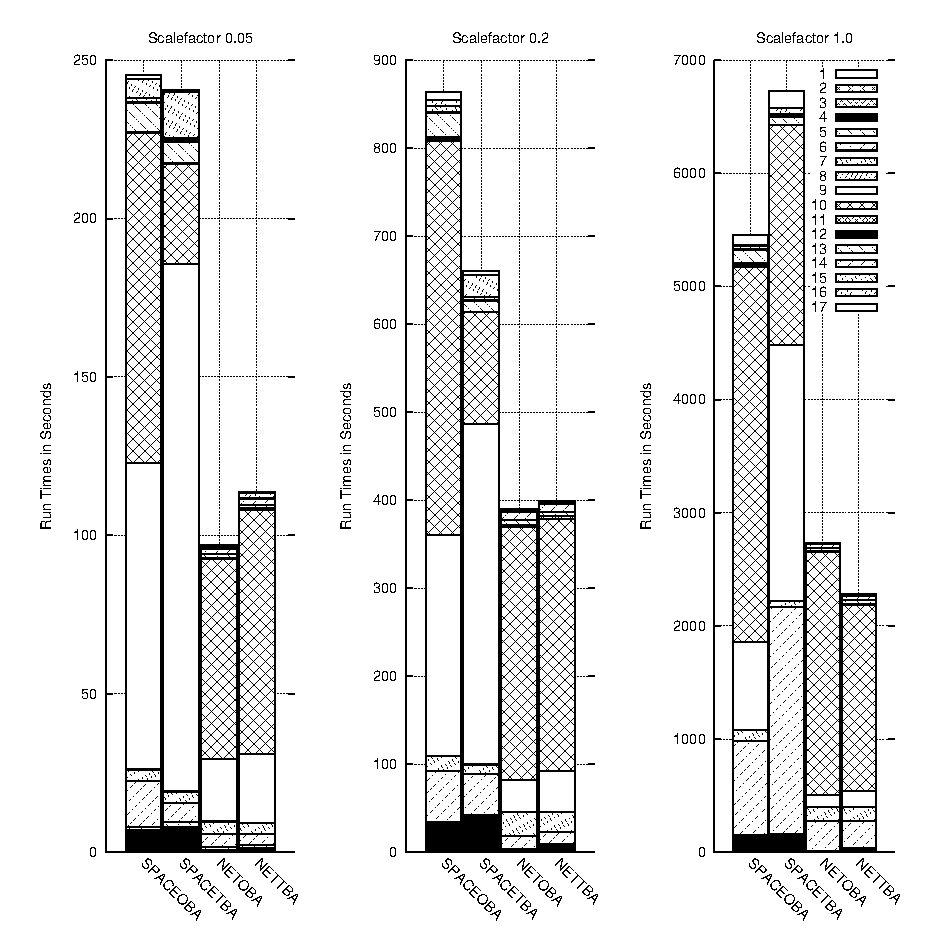
\includegraphics[width=1.0\linewidth]{compruntimesall.eps}
  \end{minipage}
 \caption{Compare Run Times}
 \label{fig:compruntimes}
\end{figure}

This can be explained by the effects of the new attributes trajectory and length
of the \dt{mgpoint} and the much lower number of units for a \dt{mgpoint} value
compared with the number of units of the corresponding \dt{mpoint} value.
In the data model of free movement in the two dimensional space every
unit must be checked to decide if a \dt{mpoint} passed a given position.
In the network data model we can do a binary check of the much
lower number of sorted $route intervals$ in the trajectory of the \dt{mgpoint}.
This effect is enhanced by a specialised network position index on this
$route intervals$ of all \dt{mgpoint} values, which is also much smaller than
the corresponding spatial index of the \dt{mpoint} values.
This effect becomes bigger as the number of cars and units grows, especially if the
observed cars drive several times the same route, like they do in the \bmodb{}
for the work trips. This effect can be seen if you compare the run times of the
queries 4, 6, 13, 15, and 16 at the different scalefactors.

The queries 8 and 9 take profit from the new length attribute of the \dt{mgpoint}
the attribute takes very small storage space compared with the trip data of a
\dt{mgpoint} but reduces the computation time of driven distances from O($n$) to
O(1) if $n$ is the number of units of the \dt{mgpoint}. The advantage can be seen
very good if you compare the different run times of query 9. While the data model
of the \bmodb{} has to add the length of each unit of the $n$ \dt{mpoint}, which
takes O(n) time, the network data model returns the driven distance in O(1) time.
The advantage is bigger for bigger scalefactors.

Interesting is also the comparision of the run times of query 10. In the object
based approach (OBA) the network data model outperforms the data model of free
movement in two dimensional space at all three scalefactors, although we do a
retranslation of the \dt{mgpoint} values into \dt{mpoint} values to use the
existing Euclidean Distance operation for \dt{mpoint} values. In
the trip based approach (TBA) the data model of free movement outperforms the network
data model at the two smaller scalfactors, while at scalefactor 1.0 the network
data model outperforms the \bmodb{} data model.

Only the queries 7, 11, and 14 show a bad performance in the network data model
compared to the \bmodb{} data model. The queries 7 and 14 use a common central
functionality to decide if a position given by a \dt{gpoint} is inside a given set of
$route intervals$ or not. This function seems to be the problem of our current
network data model implementation in \secondo{}. All other functions used by the queries
7 and 14 are also used in other queries which have a significantly better
performance.

The bad performance of query 11 is not so simple to explain. Query 12 extends query 11,
such that we expected the runtime of query 12 to be longer than the the runtime
of query 11. But the experimental results are contrary. In our experiments we
detected that the run time of a query are influenced by cache effects depending
on the environment of the single query. Such that depending of the query in a
sequence of queries the run time for the single query changes. While query 11 is not
supported by cache effects in combinatino with query 10, query 12 is supported by
cache effects from query 11. The run time differences are not so big compared to
the total run time of all queries that the very good total result would be
significantly changed by a little longer run time of query 12.

%\begin{figure}[H]
%\begin{center}
%   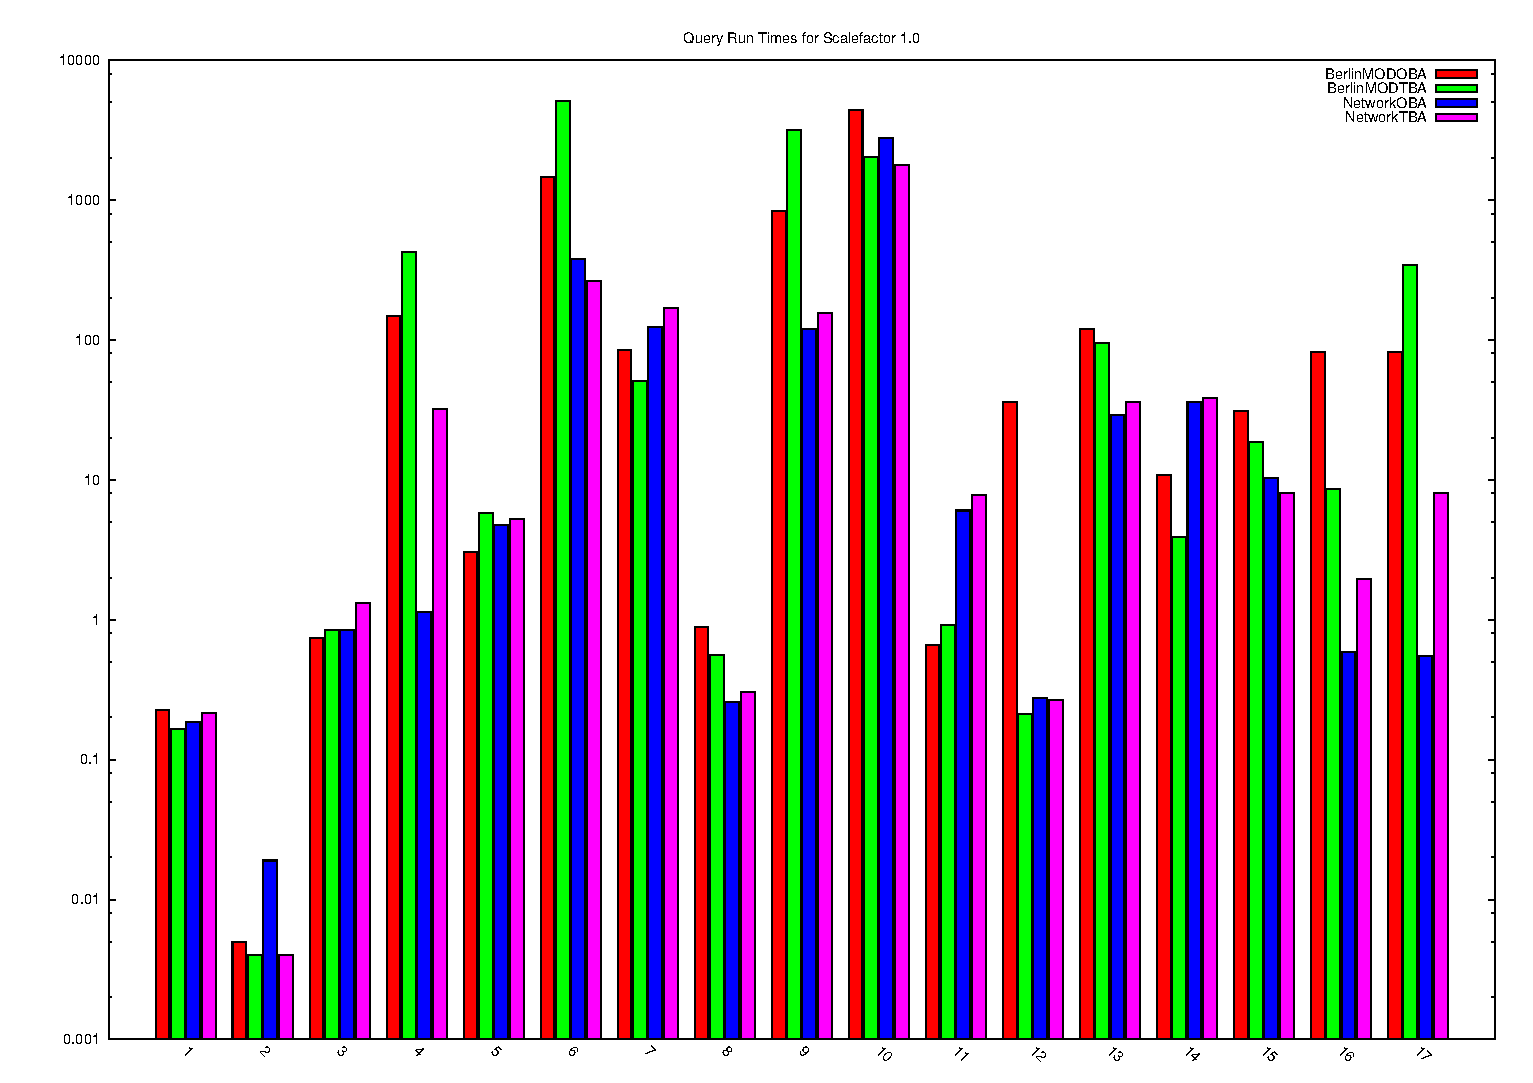
\includegraphics[width=1.0\textwidth]{compqueryruntimes.eps}
%   \caption{Compared Run Times for Each Query at Scalefactor 1.0}
%   \label{fig:compqueryruntimesall}
%\end{center}
%\end{figure}

%\section{New BerlinMOD Queries}
%\label{sec:newqueries}
\section{Summary and Future Work}
\label{sec:summary}
We presented our translation of the \bmodb{} into the network data model and
compared the capabilities of the both data models, with very good results for the
network data model. Our experiments showed that the network data model outperforms
the data model of free movement in the two dimesional space by orders of magnitudes
with respect to storage space and query run times.

The good results of the network data model encourages us to work on a extension
of the \bmodb{} to enable us to compare the capabilities of different spatio-temporal
network data models with respect to the special challenges of network data models,
like shortest path and fastest path computation. Which will be presented in near
future.

Other directions of our actual work is data mining and aggregation in our network
data model to examine traffic flow, and detect and represent traffic jams.

Other interesting themes for future work on the network data models is the efficient
computation of network distances especially between moving network objects.

\bibliography{BerlinMODAndNetworkDataModel}{}
\bibliographystyle{plain}
\end{document}
